 



\section{Data visualization}  

To explore more on how the techniques perform, we visualize the generated data by projecting them onto lower dimension space (i.e., one and two dimensions) using the Principle Component Analysis technique (PCA) \cite{pca}. Data's 2-Dimension (2D) plots and 1-Dimension histograms are presented with a hard-to-differentiate ratio (HDR) for each technique. 1D histograms are computed by dividing one-dimensional-reduced data into 20 bins (intervals) and counting the number of samples within the interval of each bin. A hard-to-differentiate ratio is defined as the ratio of the number of samples in the intersection between 2 classes to the total of minority samples ($HDR = \frac{No.\: Intersection \: samples}{No. \: Minority \: samples}100\% $) where the number of intersection samples is estimated by counting samples in the overlapped bins between the two classes in the 1D histograms. This ratio is expected to be as small as 0\% if the two classes are well separated; in contrast, 100\% indicates that the two classes cannot be distinguished in the projected 1D space. Besides HDR, we show the absolute numbers of Minority, Majority, and Intersection samples for each technique in the bottom tables. From the plots, we observe how the data are distributed in 2D space and quantify samples that are hard to be differentiated in the 1D space histograms.       


To save space, we only show the plot of one dataset (i.e., Abalone9-18 dataset) in Figure \ref{fig:visualization1d2d}. Many other datasets are observed to have similar patterns. We observe that the proposed technique does not poorly generate synthetic samples as many as other techniques do. HDR results show that \Methodname{} achieves the least number of hard-to-differentiate ratio at 15.47\%. As shown in the 2D visualization sub-figures, other techniques poorly-place synthetic data crossed the other class. This causes by outliers or noises near the border between the two classes that other techniques do not pay attention to and mistakenly create more noise. In contrast, \Methodname{} safely produces synthetic data towards the minority class by maximizing the posterior ratio ;thus it can reduce the number of poorly-placed samples.

\begin{figure*}[h!]
	\centering
	%[trim=left bottom right top, clip]
	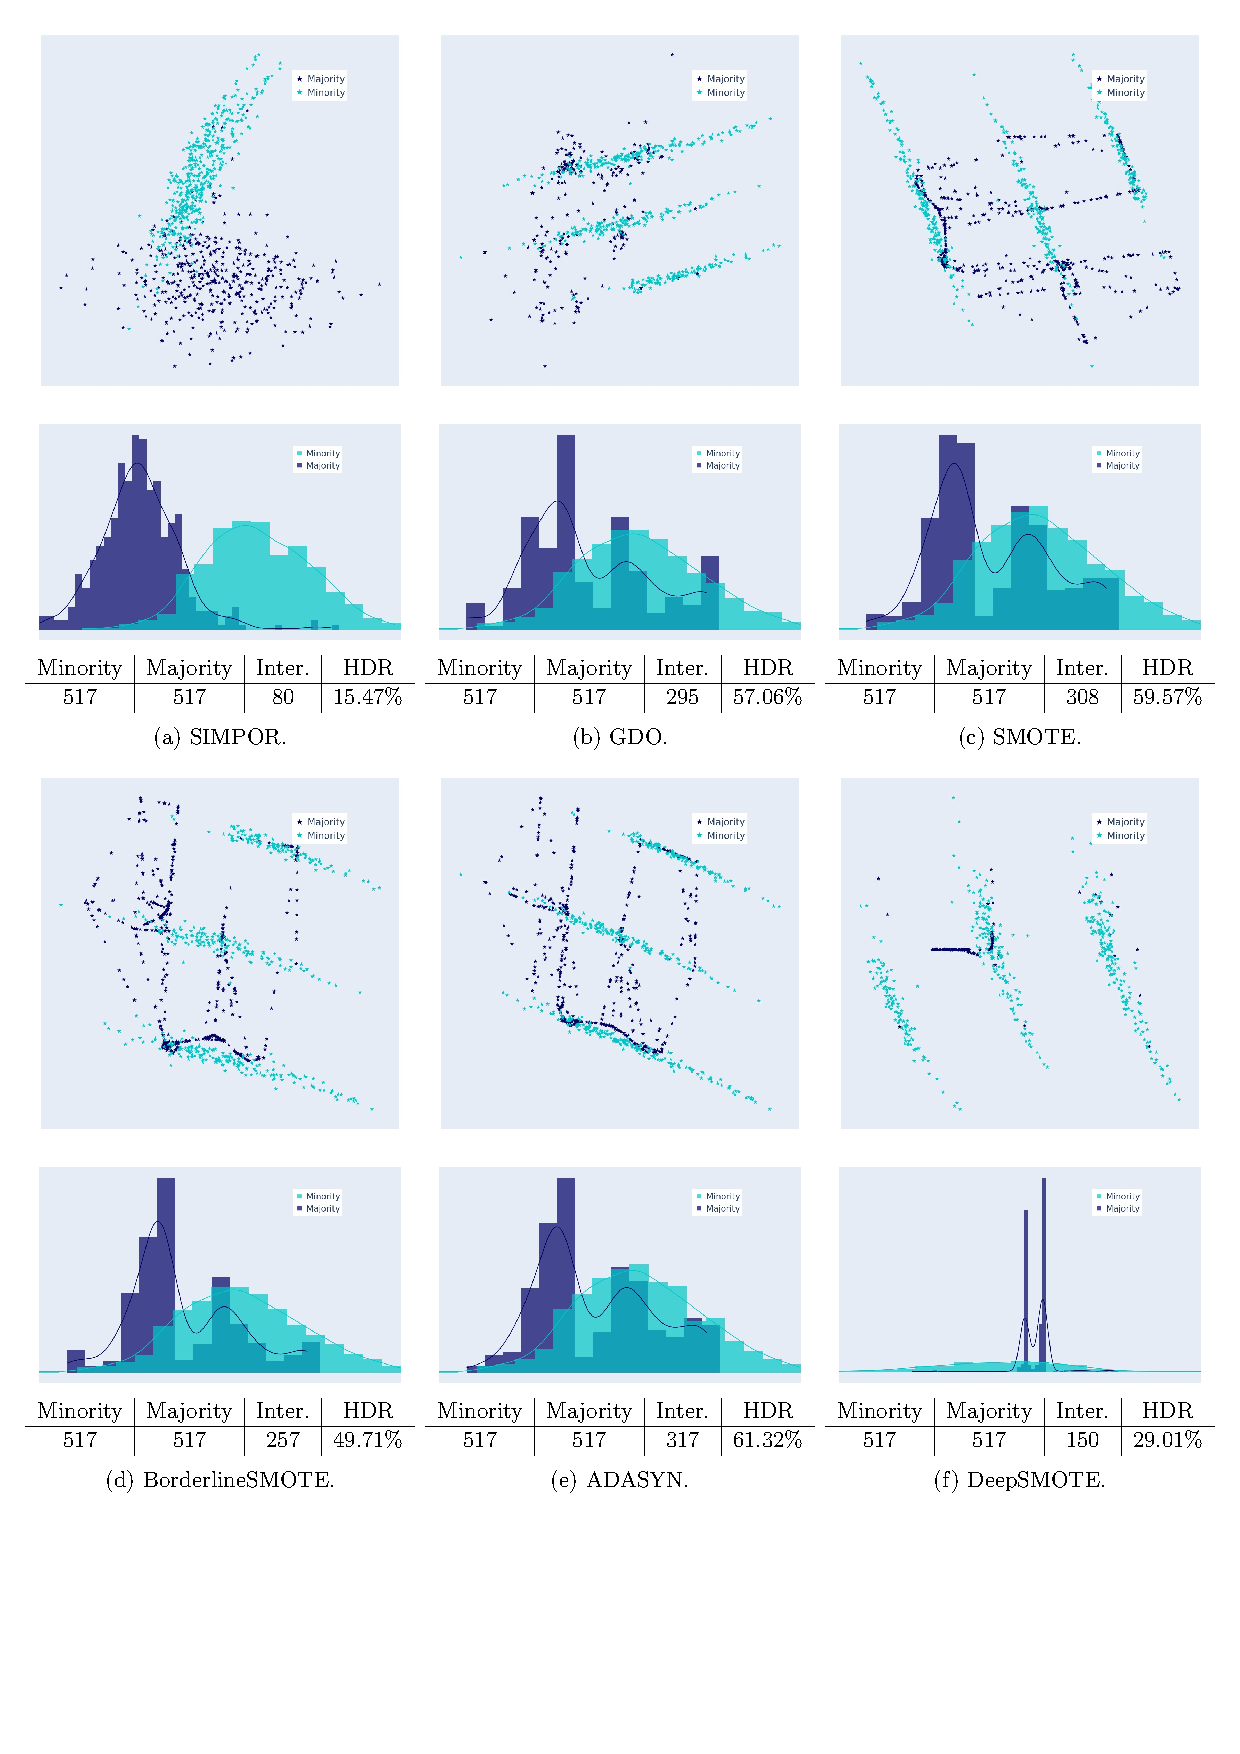
\includegraphics[width=0.8\linewidth,trim=10 90 10 10, clip ]{Figures/PCA/abalone9-18}
	\caption{Abalone9-18: Generated training data projected onto 2-dimension space and their histograms in 1-Dimension space using Principle Component Analysis dimension reduction technique. The bottom tables illustrate the number of samples in two classes, 1-Dimension histogram intersection between 2 classes, and the hard-to-differentiate ratio between the number of intersection samples to the number of minority samples ($HDR = \frac{Inter.}{Minority}100\%$).}
	\label{fig:visualization1d2d}
\end{figure*}
